\begin{figure}[htbp]
\centering
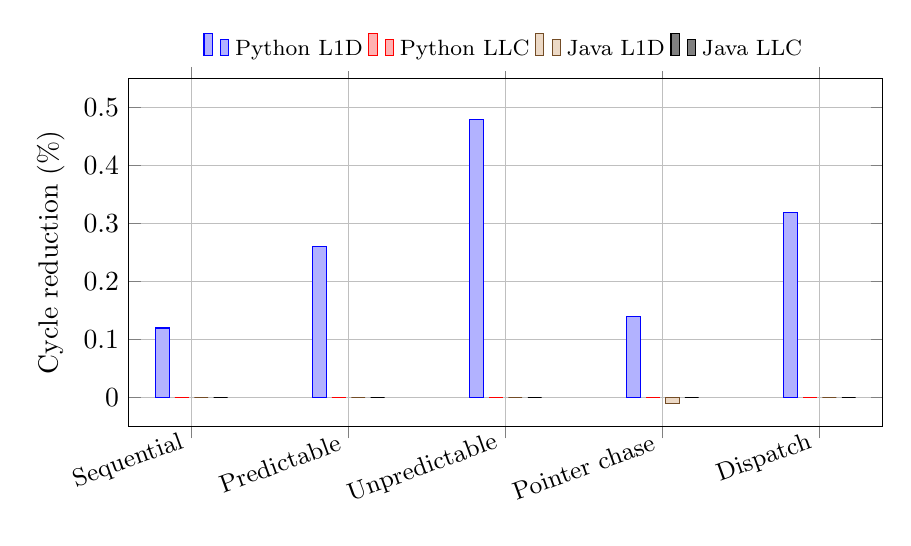
\begin{tikzpicture}
\begin{axis}[
  width=0.92\textwidth,
  height=6cm,
  ybar,
  bar width=5pt,
  symbolic x coords={Sequential,BranchPredictable,BranchUnpredictable,PointerChase,DynamicDispatch},
  xtick=data,
  xticklabels={Sequential,Predictable,Unpredictable,Pointer chase,Dispatch},
  x tick label style={rotate=20,anchor=east,font=\small},
  ylabel={Cycle reduction (\%)},
  ymin=-0.05, ymax=0.55,
  ytick={0,0.1,0.2,0.3,0.4,0.5},
  grid=major,
  legend style={at={(0.5,1.02)},anchor=south,legend columns=4,draw=none,font=\footnotesize},
]
\addplot coordinates {(Sequential,0.12) (BranchPredictable,0.26) (BranchUnpredictable,0.48) (PointerChase,0.14) (DynamicDispatch,0.32)};
\addplot coordinates {(Sequential,0.00) (BranchPredictable,0.00) (BranchUnpredictable,0.00) (PointerChase,0.00) (DynamicDispatch,0.00)};
\addplot coordinates {(Sequential,0.00) (BranchPredictable,0.00) (BranchUnpredictable,0.00) (PointerChase,-0.01) (DynamicDispatch,0.00)};
\addplot coordinates {(Sequential,0.00) (BranchPredictable,0.00) (BranchUnpredictable,0.00) (PointerChase,0.00) (DynamicDispatch,0.00)};
\legend{Python L1D,Python LLC,Java L1D,Java LLC}
\end{axis}
\end{tikzpicture}
\caption{Cycle reduction after increasing one cache's capacity by four times. Positive values mean fewer cycles.}
\label{fig:cache-sensitivity}
\end{figure}
